\chapter{Original methodology for a computer aided forensic audit}
%\komentar{Jsem si vedoma, ze jsem clovek, ktery to nikdy nedelal (= omezena znalost).
%Toto je jak to chapu. Toto neni jak by to nekdo mel delat. Toto je seriozni pokus popsat proces forenzniho auditu.
%PROCESNI DIAGRAMY!!!
%
%vystupem = okomentovany obrazek, ktery dava hlavu a patu
%
%s Use case diagrammem pak kontaktovat praxi
%
%}


We are aware to have only limited knowledge of forensic audit and no practical experience. This chapter should not be considered as a manual explaining how forensic audit should be done.  However, this is rather a serious attempt to describe the process of forensic audit.


%=====================================================================================
\section{Preparation of the process of forensic audit}
Before the process of forensic audit starts there is a block of organizational or administrative affairs that needs to be done. It all starts in an institution where there is a suspicion of an act which is not following required rules. The institution can be of various kinds. For example it can be an international corporation suspecting one of its local branches of a money leakage. %\komentar{dalsi priklady?}

The rules might be either internal regulation, corporate policies or even law. Basically suspicion of any kind of misbehavior can be investigated by forensic audit. Given the background of the case, the ordering party might also be from various branches of economy. They usually suspect possible internal or external risks that can be represented by fraudsters or people committing some other type of crime.  Generally the ordering party is the head of a given company. Some specific cases are: CEO of certain company, new holder of an existing company, authorized representative of a supervisory board etc.. However, forensic audit can be also assigned by a court or the police. 

After the decision to perform forensic audit the ordering party contacts the audit company and they negotiate with a business representative about the sphere of the contract, price and deadlines. If there is no agreement it is probable that the ordering party contacts another audit company. It is important to familiarize the ordering party with the fact that while conducting forensic audit the auditors might need access to various confidential information concerning the ordering company. On the other hand the audit company promises to manipulate with this data in a protective way and not to expose it to the risk of misuse. If all parties agree with the conditions the contract is made and the case is accepted. 

The audit company has a team of specialists established according to the character of the case. It is important to be aware of conflict of interest in this phase. Members of the team must not be related in any way to the original case. Members of the team can be forensic auditors, data analytics, specialists in any particular field (biometry, data recovery, criminology, law, etc.), consultants and assistants. 

When the team of auditors is established the next step is to create a document for record of the investigation. It also serves as documentation. It is also common to create a nickname for important subjects and for the case to provide security of the confidential information. This is the end of all the administration that needs to be done before the actual forensic audit. %\komentar{tahle posledni veta je oskliva a taky docela pochybuju, ze by se toho nedalo najit vic, co je jeste potreba udelat. Co takhle podepsat nejaky prohlaseni o mlcenlivosti nebo tak neco?}

%=====================================================================================
\section{Accumulation of data}
In the beginning of the investigation the team needs to gain an insight into the background situation of the case. They can learn it from the materials they have been provided with the client. An appropriate strategy for investigation is created. It means that all the relevant methods are taken into account of and the best ones are chosen. 

In all the cases it is important to secure all the documents, data repositories and all other possible sources of (digital) evidence. No unauthorized person is allowed to manipulate with any possible evidence. For this reason a backup of all the digital data is made. According to a FBI statistic the average investigated case size is approximately 500 GB. \komentar{citace (ariu- paper, zdroj 13)} In fact there are usually two copies of the data. The first is only for backup and the second can be used for analysis and other work with the data. 

The investigating team needs to evaluate all possible available sources of important information, access and gain the data. If the case is somehow special an expert might be needed to be authorized to collect specific pieces of evidence. An example could be a case in which a fingerprint recording is needed. 

It might be useful to visit the workplace of the investigated company and check if there are some other possible sources of evidence. After having all the data secured it can also be beneficial to perform a cross examination in some cases . It can even be done by mere conversation with involved persons, but the dialogue should be recorded.

It is possible that already in the end of collection of data the forensic audit team has a idea or even hypothesis about what happened in the case. Having this idea might be useful in further investigation. On the other hand auditors should beware of jumping into conclusions. All the actions and also any potential hypothesis should be documented in the case documentation. 

%=====================================================================================
\section{Examination}

The examination phase comes when all the data is collected. Methods of examination are very different according to the character of the case, the sources of data and also the field that is investigated. 

In the examination phase it is necessary at first to assess the data and mine the relevant pieces of information from all the collected data. It starts by identification of the data files that contain information of interest. Forensic auditors must not be discouraged by the size of data. After those files are identified it is often demanded to filter the extraneous information and leave only the coarsely filtered data. 

%=====================================================================================
\section{Analysis}

The most extensive part of the investigation comes after the data is pre-filtered. The aim of analysis is to study and analyze the data to draw conclusions from it or to determine that no conclusion can be drawn. By the end of analysis most important subjects, events, people, and people and relationships between them should be recognized. In order to find the conclusion it is required to unite information gained from multiple sources of data.

However first of all specific sources of data need to be analyzed by a competent specialist to obtain the information hidden in the data. For example, provided that a file contains billing data, the task is delegated to accountancy specialists. They can use appropriate accounting software or extract only data of particular interest and use some quantitative software. If the data contain log files or deleted files it is a job for information technology specialists to recover or examine the data. 


Some of the methods the team of investigators might use are: quantitative analysis, analysis of relationships between persons, making use of analytical software. \dotaz{Jake jsou ty metody?} In case of  suspicion from corruption an investigation of decisions made by the management of the company might be needed. Investigators might pose questions similar to following: Who are the suppliers of the investigated company? In what business the company invests and who makes the decisions about it? Who does have an access to (financial) resources?


There might be cases when specialists in various sub-branches of forensics might be needed. Even an external company might be hired to solve a particular problem. Examples of auxiliary specialists can be experts in computer forensics, forensic dactylography, digital forensics, forensic biometry, forensic psychiatry, forensic linguistic etc. According to opinions of all available experts the situation in the case is gradually revealed.

All the steps taken in the analysis result in understanding of the situation in the case. A verdict is pronounced according to the information investigators gained and it is retrospectively supported by the data collected in the beginning of the process. 


%=====================================================================================
\section{Reporting}

After having investigated the assigned case the team of forensic auditors has some results to show. Either they have found what undesirable actions happened or there might be cases when they have not discovered any signs of such behavior. In both cases the results are presented to the ordering party. 


There are multiple possible results of previous investigations. Basically either a suspicion has been confirmed or it has not. If the investigation discovered a crime the exact methods that lead to the discovery must be mentioned in the report together with the evidence supporting the result. The report should clarify if there is enough evidence. If there is not enough evidence the type of data needed to prove the result should be described and reasoned. The explanation why there is no evidence yet should be also given.


If no crime has been discovered in the reporting stage, it still must be explained in the report what data has been investigated and how the investigation was conducted. Everything that has been found out about the case should be presented in an appropriate form. Special effort should be made in presenting possible alternative explanations. One of them might be that there has not been enough time to process all available data. In that case it leads to a customers decision. They decide whether they want to continue the investigation in more details or whether they are content with the result and they already believe that no crime has been committed. This situation is very case-specific. 

According to the result of the investigation several additional information might be suggested. This might be for example an advice about subsequent actions preventing repetition of the undesirable behavior. While investigating a case forensic auditors might sometimes discover a completely new problem in the investigated company. This additional information should be also included in the report. 

The actual reporting is affected by many factors. When preparing the final presentation these factors should be considered. First, the presentation should be prepared with regard to the audience the speaker is going to have. The extent of professional details regarding the methods used in the process should be adjusted to the anticipated knowledge of the audience. However, if asked, the speaker should be prepared to explain the details. The presentation should be easily comprehensible and explain everything discovered in the investigation. 

One part of the report can be focused on alternative explanations of what happened. This may happen if the information that has been found about an event is incomplete. Alternatively it may happen if there are more plausible explanations about what happened. Each of these explanations should be analyzed in the previous phase and an attempt to prove or disprove them should be made.


Besides an oral presentation the output of the assignment should be also a written document describing all the important facts about the case. This document should be handed over to the ordering party and should contain:
\begin{itemize}
\item information about the agreement between the two sides,
\item list of sources of evidence in the investigation,
\item description of methods used in the investigation,
\item the sequence of important evidence found in the data,
\item explanation of the evidence,
\item summarization of what the evidence results in,
\item recommendation on how to prevent similar future situations,
\item optionally suggestions what steps should be taken to improve the current state,
\item conclusion of the case.
\end {itemize}


In the end of the reporting stage the forensic audit is either concluded or a decision on further investigation is made and precise conditions specified. Forensic audit is concluded if the particular crime has been revealed and evidence supporting this is found. Alternatively it might be concluded if all the information about the case suggests that no crime has been committed. Another possibility is when the ordering party for some reason does not want to continue the investigation. 

On the contrary if there is still a suspicion that a crime has been committed the investigation might continue after reporting stage. This can happen if a suspicion on a new crime has emerged. The investigation also continue if it is expected that the evidence supporting the crime might be found soon if given more effort. If decided so, the investigation might continue from any of the previous steps forwards. 

%\anglictina{
\section{Work following after a forensic audit}
%}

When the process of forensic audit ends both the ordering party and the audit company do a follow-up work. The ordering party usually uses the results of forensic audit for their own benefit. They can use the evidence gathered during the forensic audit in court of justice. They can also use it to prevent similar scenarios from happening or eliminate the source of this behavior. This can mean to fire an untrustworthy employee or change the rules or internal policies. 

Follow-up work in the audit company applies mainly to extension of experience and expert's opinions in the audit company. Such company usually has more than one team and works on multiple cases at the same time. Improving their knowledge is an important part of their development. On the other hand the audit company must respect confidentiality of the information about the case and guarantee its unconditional anonymity.

%Another type of follow-up work might be considered continuous education in newest trends in the field, technologies and legislation as well.
%Tenhle "jinej typ prace" je stejnej, jako to sebevzdelavani se v predchozim odstavci.

\colorbox{green}{\komentar{ timhle diagramem bude problem, budu ho muset prinutit aby se rozdelil na vic stran}}

\begin{figure}[h]
	\begin{center} 
	%\missingfigure{Velky obrazek vsech zainteresovanych stran - f.auditor, datovy analytik pro FA, zakaznik (zadavatel, materska spolecnost)}
	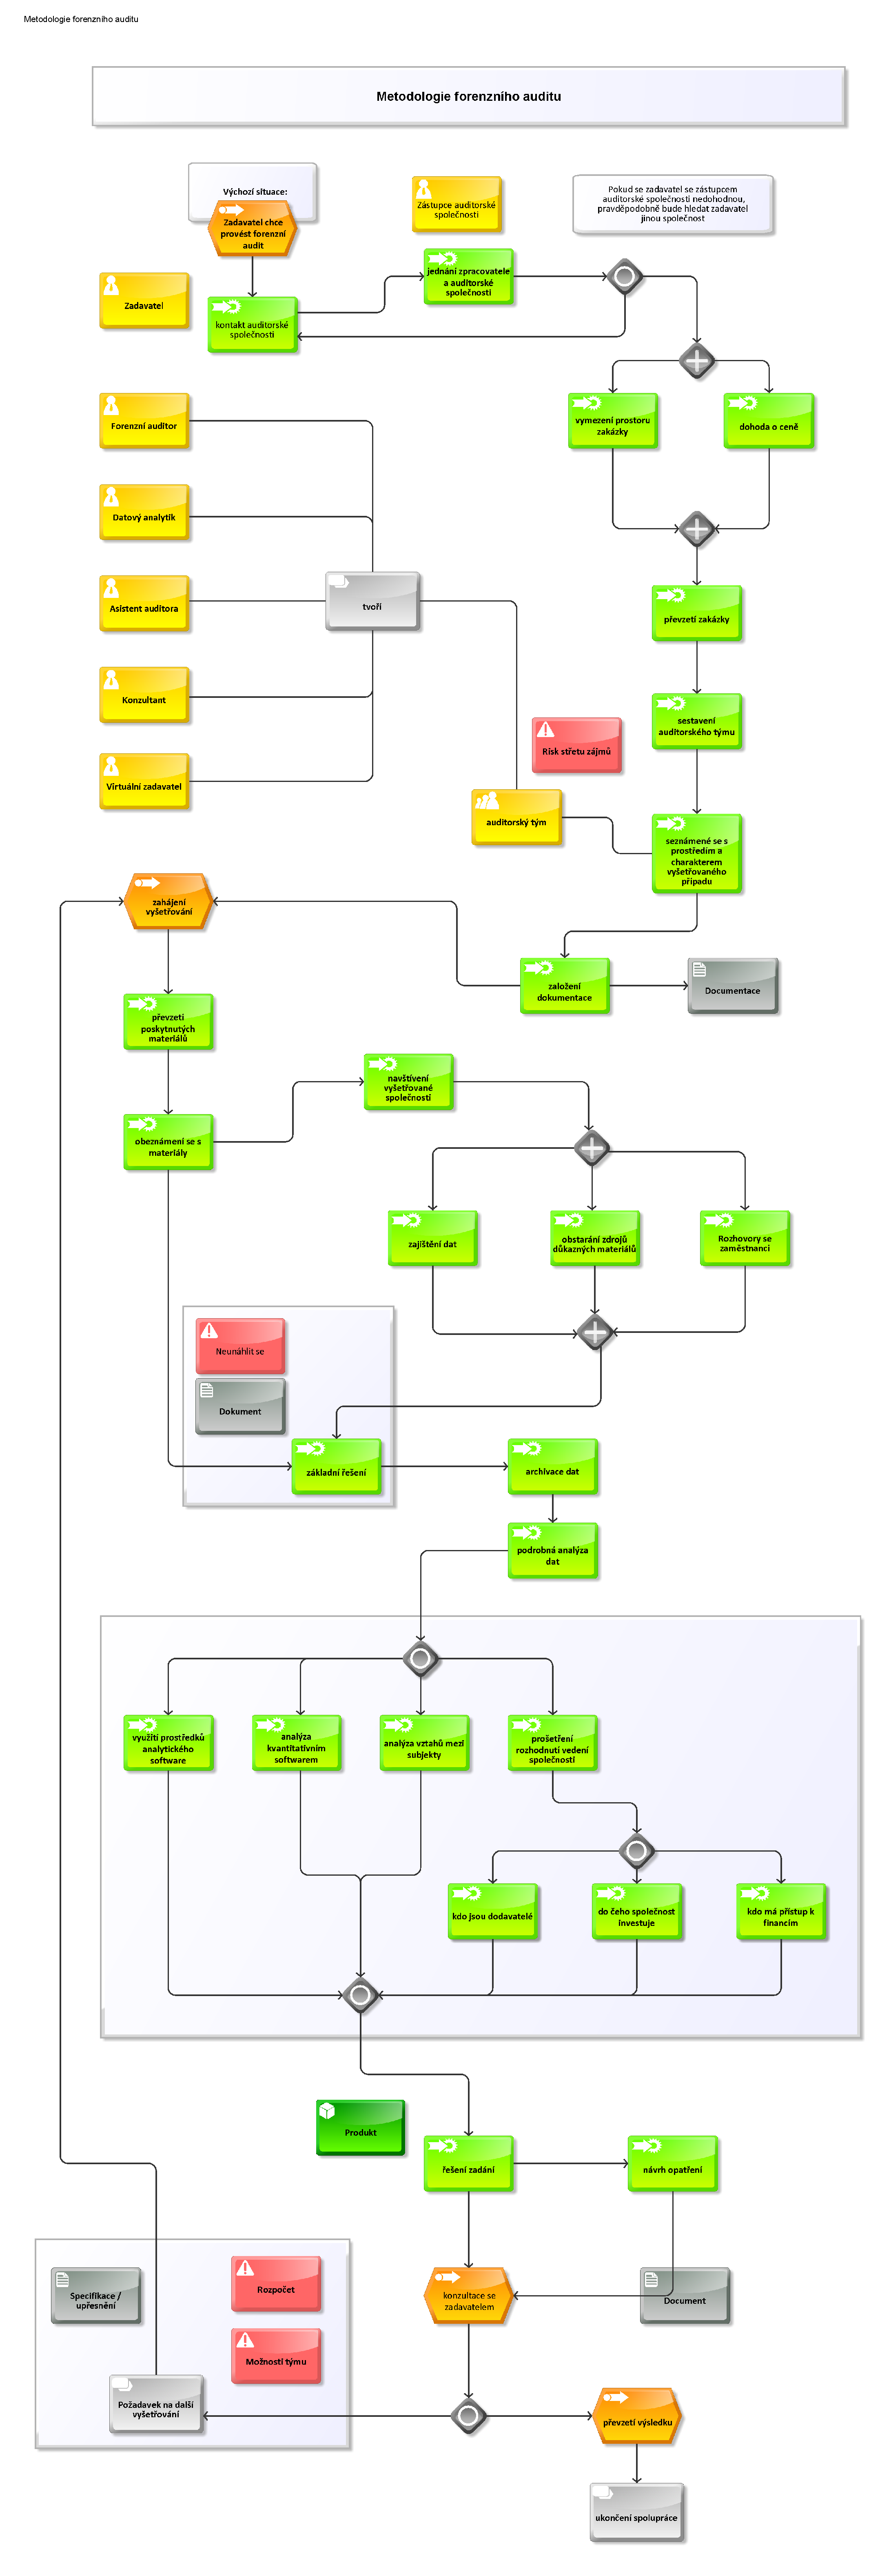
\includegraphics[width=1.0\textwidth]{img/metodika/Metodologie_forenzniho_auditu.pdf}
	\end{center}
	\caption{\komentar{Metodika v ARISu}}
\end{figure}

 
